
Para poder realizar las simulaciones en \cw\ se ha trabajado con una corriente de inyección constante e igual a la corriente de polarización ($I(t) = I_{bias}$), tomando $V_{RF} = 0$.

Se pueden obtener expresiones anal\'iticas en el estado estacionario para $N(t)$ y $S(t)$, $N_0$ y $S_0$ haciendo $\frac{\mathrm{d} N}{\mathrm{d} t} = \frac{\mathrm{d} S}{\mathrm{d} t} = 0$ \cite{van1995semiconductor}. Para el caso de $N(t)$ se obtiene el resultado sencillo de $N_0 = N_{th}$. Para el caso de \s, esta constante es igual $S_0 = cte (I- I_{th})$. En estas condiciones la fase cambiará linealmente con el tiempo, haciendose cero en el caso de que corriente sea la corriente umbral.

\addtocontents{toc}{\vspace{0.1cm}}
\subsection{Espectros de emisión}
	\label{Sol:CW:Spectr}

	Es importante conocer el valor de la longitud de onda del pico de emisión del láser en solitario en función de la corriente de polarización $\ibias$, de cara a realizar el estudio de la inyección de luz.

	En la Figura \ref{Img:spectrosCW} se muestran las densidades espectrales de potencia del láser a diferentes corrientes de polarización, comparando los datos obtenidos mediante la simulación del láser(Figura \ref{Img:spectrosCW:sim}), con los obtenidos experimentalmente(Figura \ref{Img:spectrosCW:exp}).

		% Img:spectrosCW {Img:spectrosCW:sim, Img:spectrosCW:exp}
		\begin{figure}[H]
			\centering
			\begin{subfigure}{0.45\textwidth}
				\centering
				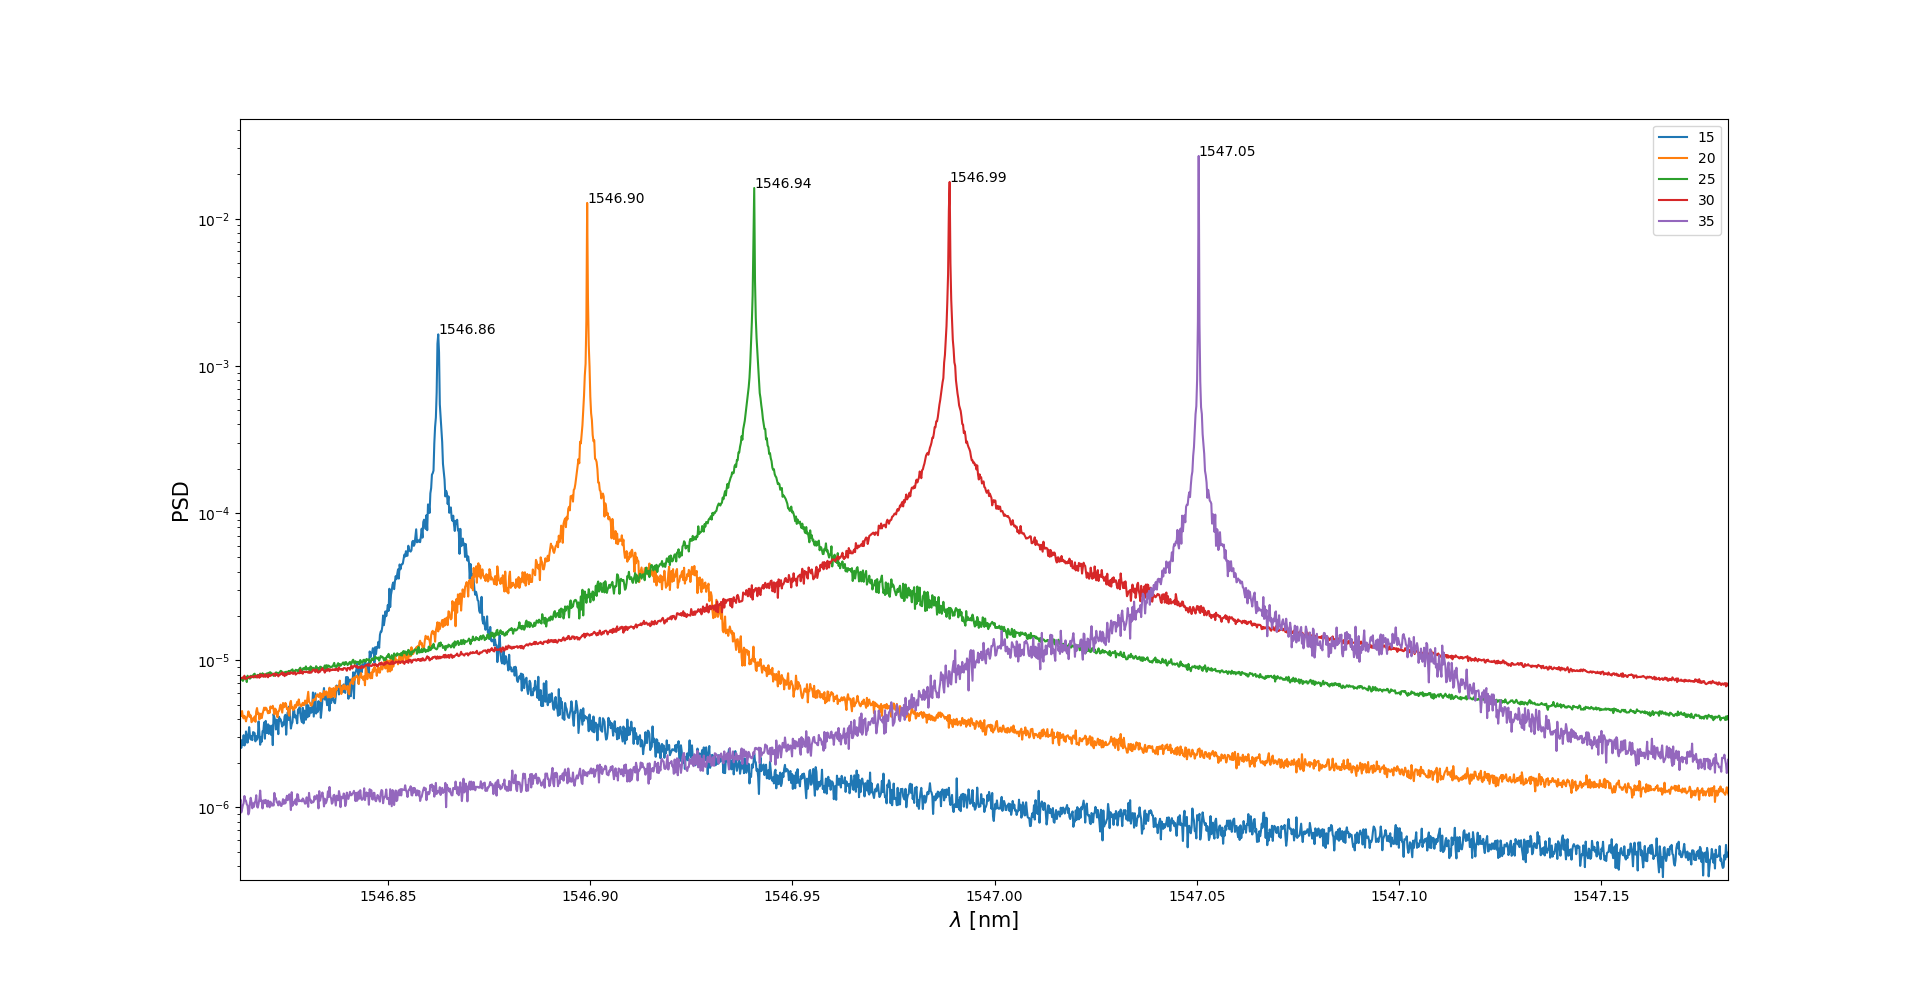
\includegraphics[width=1.0\linewidth, height=6cm]{Espectros.png}
				\caption{\label{Img:spectrosCW:sim}Espectros ópticos obtenidos mediante simulación para distintos valores de la corriente.}
			\end{subfigure}
			\begin{subfigure}{0.45\textwidth}
				\centering
				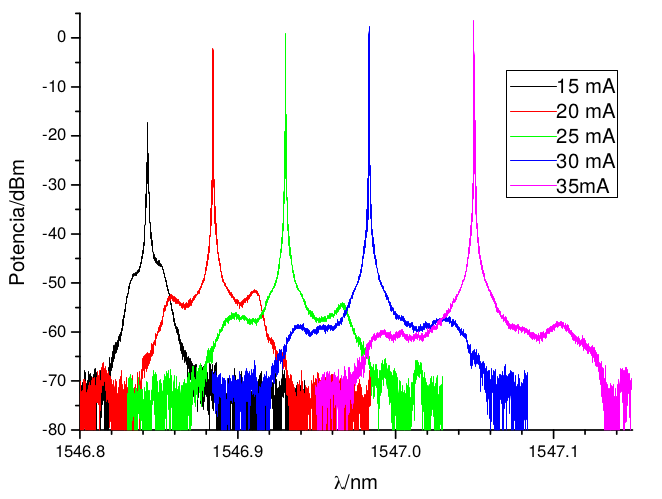
\includegraphics[width=1.0\linewidth, height=6cm]{../Chaves/OFC-GS/espectros_continua.png}
				\caption{\label{Img:spectrosCW:exp}Espectros ópticos obtenidos experimentalmente para distintos valores de la corriente.}	
			\end{subfigure}
			\caption{\label{Img:spectrosCW}Espectros ópticos del DML para diferentes corrientes de polarización $\ibias$ obtenidos mediante simulación (izquierda \ref{Img:spectrosCW:sim}) y mediante experimento (derecha, \ref{Img:spectrosCW:exp}).}
		\end{figure}

		Comparando los espectros obtenidos mediante simulación con los obtenidos experimentalmente se observa un gran parecido en la forma. Se observa además un corrimmiento hacia el rojo y un aumento de la potenica óptica, a medida que aumenta la corriente. El corrimineto hacia el rojo se debe a efectos térmicos: Al aumentar la corriente aumenta la temperatura de la región activa, por efecto Joule, debido a la resistencia eléctrica del dispositivo. En semiconductores el índice de refracción aumenta con la temperatura y por tanto la longitud de onda de resonancia aumenta con la corriente \ref{eq:Cond}. Además, la simulación permite observar los picos propios de las oscilaciones de relajación del láser que se observan en el experimento. Estos picos son los picos satélites que aparecen al rededor de la línea dominante, correspondiendo la diferencia de frecuencias ópticas entre el pico satélite y el pico dominante a la frecuencia de las oscilaciones de relajación \cite{van1995semiconductor}.

			\begin{equation}
				\lambda_0 = \frac{2nL}{q}
				\label{eq:Cond}
			\end{equation}

		Además, a partir de los espectros de la Figura \ref{Img:spectrosCW} se pueden obtener las longitudes de onda de los picos de emisión en función de la corriente $\ibias$. En la Tabla \ref{tab:lambdas} se muestran los valores de las longitudes de onda $\lambda$ obtenidas de los espectros de la Figura \ref{Img:spectrosCW} tanto para la simulación como para el experimento.

		% tab:lambdas
		\begin{table}[H]
			\centering
			\begin{tabular}{c c c}
				\hline
				$\ibias$ [mA] & $\lambda_{sim}$ [nm] & $\lambda_{exp}$ [nm] \\\hline 
				15 & 1546.86 & 1546.84 \\
				20 & 1546.90 & 1546.88 \\
				25 & 1546.94 & 1546.93 \\
				30 & 1546.99 & 1546.98 \\
				35 & 1547.05 & 1547.05 \\\hline
			\end{tabular}
			\caption{\label{tab:lambdas}Longitud de onda de las lineas de emisión del DML en función de la $\ibias$ obtenidas de la figura \ref{Img:spectrosCW}. Se muestran los valores experimentales $\lambda_{exp}$ obtenidos de la gráfica \ref{Img:spectrosCW:exp}, y los valores obtenidos de la simulación de la gráfica \ref{Img:spectrosCW:sim}.}
		\end{table}

	Los valores de las longitudes de onda que se muestran en la Tabla \ref{tab:lambdas} muestran una gran similitud entre los valores experimentales y los obtenidos mediante simulación, obteniendo una discrepancia máxima de $0.02$ nm. De esta forma, la buena concordancia entre los valores de $\lambda$ experimentales y los obtenidos a partir de la simulación, junto con la gran similitud en la forma de los espectros, muestra la capacidad de la simulación de reproducir computacionalmente los resultados obtenidos experimentalmente en el laboratorio.

	Para el estudio de la inyección de luz se trabajará con una corriente $I_{bias} = 35$ mA. Por tanto, la Tabla \ref{tab:lambdas} permite obtener su longitud de onda de emisión de $\lambda = 1547.05$ nm, siendo además la misma que la obtenida en el experimento.

\addtocontents{toc}{\vspace{0.1cm}}
\subsection{Oscilaciones de Relajación}
	\label{Sol:CW:RoF}

	Para que el láser comience a emitir se ha de cumplir que la emisión estimulada domine frente a la emisión espontánea. Esto se produce cuando la corriente inyectada en la región activa supera un valor umbral, $I_{th}$, a partir del cuál el láser comienza a emitir una cantidad apreciable de fotones por emisión estimulada. Si la inyección de corriente que se le aplica al láser es constante (\cw), la densidad de portadores de carga tenderá a estabilizarse en $N_{th}$. Del mismo modo, la densidad de fotones se estabilizará para valores $S_{0}$ y el $\nu_{chirp}$ para valores de $C(I)$.

	Si se parte de unas condiciones iniciales del láser con valores $N(t=0) < N_{th}$, será necesario que transcurra un cierto tiempo hasta que el láser alcance un estado estacionario en el que las variables alcanzan valores constantes. A este tiempo se le denomina transitorio.

	%Cabe destacar que, tal y como se comentó en el apartado \ref{Mdl:Code:Trans}, para la simulación se ha trabajado con un tiempo de transitorio $t_{trans} = 1.2$ ns, en el cuál se ha operado con la raiz cuadrada del módulo de $S$ en los términos de ruido para evitar resultados complejos, despeciando dicho intervalo en el estudio de los espectros. Sin embargo, en este apartado se estudiarán las ecuaciones de balance en el transitorio para corriente continua. El trabajar con una corriente continua mayor que la corriente umbral permite disminuir el intervalo de tiempo en el que se operará con $\sqrt{|S|}$ hasta los 0.2 ns, pudiendo realizar un estudio más riguroso de las ecuaciones de balance en el transitorio.

	Se considerará una intensidad de corriente $I(t)$ función escalón con $I(t>0) = \ibias$. En la ecuación \ref{eq:transient} se muestra la función escalón $I(t)$ utilizada así como las condiciones iniciales para la densidad de portadores de carga $N(0)$, la densidad de fotones $S(0)$ y de la fase óptica $\Phi(0)$.

		%eq:transient
		\begin{equation}
			\begin{matrix}
					I(t) = \left\{\begin{matrix}
									0 & t \leq 0\\ 
									\ibias = 30 \textrm{ mA} & t > 0
							\end{matrix}\right.
					& & & & & & 
					\begin{matrix}
						N(0) = N_{tr} \\ S(0) = 10^{15} \textrm{m}^{-3}\\ \Phi(0) = 0
					\end{matrix}
				\end{matrix}
			\label{eq:transient}
		\end{equation}

	En la Figura \ref{Img:transitorio} se muestra la evolución temporal de la \I\ junto con los valores obtenidos en la simulación para la \n\, la \s\ y del \chirp\ para el transitorio $t_{trans} = 1.2$ ns.

		% Img:transitorio
		\begin{figure}[H]
			\centering
			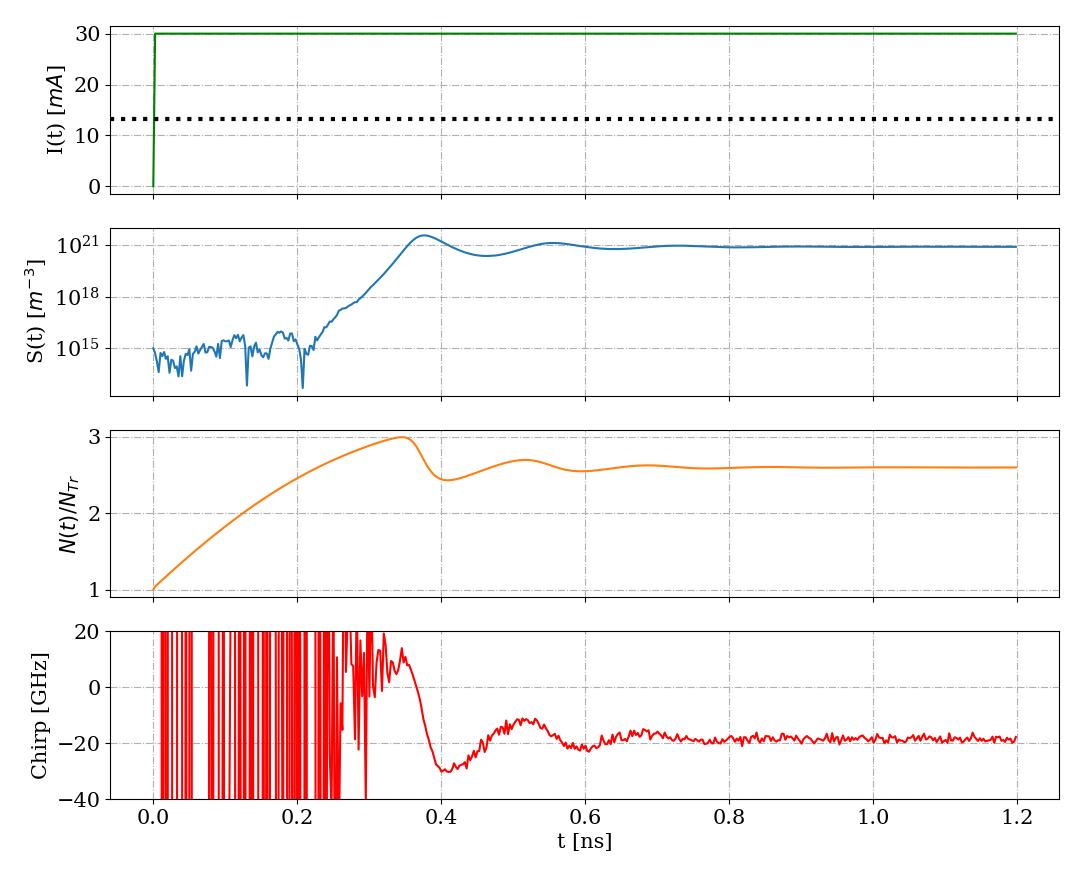
\includegraphics[width=0.7\linewidth]{transitorio.png}
			\caption{\label{Img:transitorio}Evolución temporal de la \I, la \s, la \n\ y del \chirp\ durante el transitorio. Para la \I\ se ha marcado la corriente umbral del láser $I_{th} = 14.8$ mA con una línea horizontal discontinua.}	
		\end{figure}
		
		Se observan en las evoluciones temporales de \n, \s\ y \chirp\ de la Figura \ref{Img:transitorio} tres regiones diferentes en función del comportamiento de las tres magnitudes: $i$) Una vez que la corriente inyectada supera la corriente umbral $I_{th}$ (en $t=0$) la \n\ comienza a aumentar. No obstante, el valor de $N(t)$ se mantiene inferior a $N_{th}$ por lo que no se produce emisión estimulada, y así, la densidad de fotones no aumenta y toma valores aleatorios, debido a la emisión espontánea, alrededor de $S(0)$. Esto también se puede observar en el comportamiento también aleatorio del \chirp. $ii$) La \n\ continua aumentando alcanzando el valor umbral $N_{th}$ en $t = 0.23$ ns. En este punto la densidad de fotones comienza a aumentar debido a la emisión estimulada producida al superar $N_{th}$. Sin embargo, $N(t)$ continua creciendo tomando valores por encima de $N_{th}$ hasta que sufre una disminución brusca acompañada de la emisión de un pulso de luz (ver $S(t)$ entre 0.35 y 0.45 ns). Una vez emitido el pulso $N(t)$ vuelve a crecer de tal forma que tanto $N(t)$ como $S(t)$ tienen un comportamiento oscilatorio al rededor de $S_0$ y $N_{th}$ con una amplitud decreciente. Estas oscilaciones se les llama oscilaciones de relajación. En la figura \ref{Img:transitorio} se observan claramente estas oscilaciones, estando en fase para \n\ y para el \chirp\ (máximos en el mismo tiempo $t$). También se observa la relación entre las oscilaciones de estas magnitudes con las de $S(t)$. Tienen la misma frecuencia aunque existe un desfase entre ellas, obteniendo un máximo en $S(t)$ cuando $N(t) = N_{th}$. $iii$) Las oscilaciones de relajación van disminuyendo a medida que el tiempo avanza alcanzando el estado estacionario en el que las tres magnitudes se mantienen constantes.

		A partir de los datos de la figura \ref{Img:transitorio} se pueden obtener las frecuencias de las oscilaciones de relajación en el transitorio, a partir del tiempo entre los máximos. Una primera estimación permite obtener una frecuencia de oscilación de $\nu_{RoF} \approx 5.9$ GHz, que pasado a longitud de onda equivale a $\lambda = 0.05$ nm. Comparando dicho valor con los picos debidos a las oscilaciones de relajación de los espectros para $I = 30$ mA de la figura \ref{Img:spectrosCW} observamos que se encuentran en el mismo orden de magnitud, mostrando una buena concordancia entre la simulación y el experimento.
